%%%%%%%%%%%%%%%%%%%%%%%%%%%%%%%%%%%%%%%%
%                                      %
% Athanassios Protopapas, October 2005 %
% Mini-example for using apa.cls       %
%                                      %
%%%%%%%%%%%%%%%%%%%%%%%%%%%%%%%%%%%%%%%%

\documentclass{cimento}
\usepackage{graphicx}  % got figures? uncomment this
%\bibliographystyle{apacite}
\usepackage{lineno}  % got figures? uncomment this
\usepackage{braket}
\linenumbers
\title{Statistical classification using different approaches based on the Bayes Theorem and the Quantum Mechanics formalism}

\author{F.~Noferini\from{ins:centrofermi}\from{ins:infn}}
\instlist{
  \inst{ins:centrofermi} Museo Storico della Fisica e Centro Studi e Ricerche ``Enrico Fermi'' - Rome, Italy
  \inst{ins:infn} INFN, Sezione Bologna - Bologna, Italy
  }
  
 %%The correct list of PACS numbers and definitions is available at www.aip.org/pacs/pacs2010/about.html
\PACSes{\PACSit{--.--}{\dots}
\PACSit{--.--}{\ldots}}

%\acknowledgements{Written at the request of the Prac\TeX\ journal editors. Comments may be sent to the author at protopap@ilsp.gr.}

%\shorttitle{APA style manuscript}
%\rightheader{APA style manuscript}
%\leftheader{A.\ Protopapas}

%\newcommand{\jpsi}{\ensuremath{\rm J/\Psi}}

\begin{document}

\maketitle                            
\begin{abstract}
In this work a novel statistical approach is presented.
The aim of such an appraoch is to classify events associating a probability to belong to different classes in a way
which allows to classify simultaneoulsy events both in a statistical way and on event-by-event basis.
In particular two different startegies were derived in a similar framework: one using the Bayes' theorem properties
and one using the Quantium Mechanics formalism which treats, at statistical level, the usual finite detector resolution as a quantum
wave function effect.
\end{abstract}

%\tableofcontents{}

\input{introduction}
The classification operation is a very general concept which may assume different meaning depending on the context in which
it is applied.
Here we are referring to the capability to discriminate different event classes on the basis of some
measured variables.
Because of a usual finite resolution in a single measurement different classes may be not completelly separable
in the sense that for a single event it is not possible to define with absolute certainty if it belongs to a class
or to another one.
In the case we are interested to perform measurement by selecting a specific event class there are usual two kinds of
approaches which can be exploited: a statistical approach which allows to unfold the finite resolution/spread of our
measurements to extract the number of event belonging to that class (for instance by fitting the distributions in the
variables we are able to measured); or defining some cuts on the variables which minimize the contamination of other classes.
In the first case we are able to extract the total number of events without, in principle, any efficiency loss and
contamination but we are not able to classify on event-by-event basis.
In the latter one we can associate each event to a class (useful to characterize the properties of the class in terms of
other variables/osservables) but we have to deal with corrections for efficiency loss and contamination.
The idea to associate a probability to each event is to extend the properties of the statistical approach, no
efficiency loss and no contamination by other classes, to the event-by-event approach by replacing the concept
of cut with the use of a  weight.
In this approach the probability used as a weight should guarantee that the effect of the contaminations by other
event classes goes to zero whena averaging on all the events.

In the first section we will present a general formalism to define probabilities under different assumptions
and to derive the properties in each scheme we presented.
In the second section we will focus on the two particular cases introduced before, Bayesian probabilities and Quantum probabilities,
extending the study to the multi-variable and multiple-classification scenarios.
In the third section some example will be reported to show the power and the limitations of the methods.
Finally, we will discuss our results reporting our conclusions and final remarks.

\section{Connection between statistics and event-by-event appraoch}
\subsection{The foundamental relation}
If we consider the case with a sample of data composed by $N_{type}$ classes distinuguished via the measurement of signal $S$ measured by a specific detector.
Assuming to know exactly what is the detector response for each event class expressed by $p_{i}(S)$ with i=1,2,...,$N_{type}$ and $\int p_{i}(S) dS = 1$.

A priori we don't know what the abundances, $M_{i}$, for the event classes are which is usually what we want to measure, we just know what is the total event multiplicity $M = \sum\limits_{i}^{N_{type}} M_{i}$ 
Keeping them as a variable we can define the following relation for a generic function $f(S)$ of the signal:

\begin{equation}
\label{Sec1:BasicRelation}
\sum\limits_{j}^{M} f(S) = \sum\limits_{i}^{N_{type}} M_{i} \int p_{i}(S) f(S) dS,
\end{equation}
such a relation is valid because on average the signal distribution for a given class has to be distributed accordingly to the know detector response.

It is worth to note that the relation in eq.~\ref{Sec1:BasicRelation} is valid for any function $f(S)$ depending on the signal and it is interesting to see what happens when we replacing it with some specific functions.

First of all we are going to introduce a probability defined using the Bayes theorem. Such a probability, which depends on the measured signal, was particulary used in the ALICE experiment (reference) to identify particles (in that case event classes are represented by different particles type) and therefore it was reported as a good candidate to define the probability we are looking for.

Using the Bayes theorem where $p_{i}$ represent the conditional probability (the probability that an event of a class, $H_{i}$, relases the measured signal) $P(S|H_{i})$ it is possible to derive the posterior probability (the probability that the measured signal belongs to an event of the class $H_{i}$) $P(H_{i}|S)$ via the formula (for simplicity we will refer to it simply with $P_{i}(S)$):
\begin{equation}
\label{Sec1:BayesianProb}
P_{i}(S) = P(H_{i}|S) = \frac{C_{i} P(S|H_{i})}{\sum\limits_{i}^{N_{type}}C_{i} P(S|H_{i})} = \frac{C_{i} p_{i}(S)}{\sum\limits_{i}^{N_{type}}C_{i} p_{i}(S)},
\end{equation}
where $C_{i}$ is usually called the prior probability which is the best guess of the abundances for all the event classes, expected to be as closer as possible to the the real one $M_{i}$. The main property of the Bayesian probability is that by definition $\sum\limits_{i}^{N_{type}} P_{i}(S) = 1$.

The use of Bayesian probability is applied by replacing in eq.~\ref{Sec1:BasicRelation} $f(S)$ with $P_{i}(S)$, i.e. by counting all the events with the probability as a weight. The way the Bayesian probability is defined guarantees very important properties:
\begin{eqnarray}
\label{Sec1:BayesianProp}
\sum\limits_{j=1}^{M}P_{i}(S) = M_{i},{\rm\ if\ {\it C_{i} = M_{i}}}, \\
\label{Sec1:BayesianProp2}
C_{i} \rightarrow M_{i} {\rm\ via\ iterative\ procedure}.
\end{eqnarray}
While the property in eq.~\ref{Sec1:BayesianProp} can be easily demonstrated by replacing in eq.~\ref{Sec1:BayesianProb}  $C_{i}$ with $M_{i}$, the latter one requires more extended computation.
In particular for $C_{i} \neq M_{i}$ eq.~\ref{Sec1:BayesianProp} can be rewritten (after some calculations) in the form:
\begin{eqnarray}
\label{Sec1:BayesFullCalc}
\sum\limits_{j=1}^{M}P_{i}(S) = M_{i} \int \frac{1}{1+\frac{\sum\limits_{k \neq i} \left( \frac{C_k}{C_i} - \frac{M_k}{M_i} \right) p_{k}(S)}{1 + \sum\limits_{k \neq i} \frac{M_k}{M_i} p_k(S)}} p_{i}(S)dS \sim \\
\sim M_{i} \int  \left( 1+\frac{\sum\limits_{k \neq i} \left( \frac{M_k}{M_i} - \frac{C_k}{C_i} \right) p_{k}(S)}{1 + \sum\limits_{k \neq i} \frac{M_k}{M_i} p_k(S)} \right) p_{i}(S)dS = \\
= M_{i}  \left( 1 + \sum\limits_{k \neq i}  \left( \frac{M_k}{M_i} - \frac{C_k}{C_i} \right) \int  \frac{p_{k}(S)p_{i}(S)dS}{1+\sum\limits_{l \neq i} \frac{M_l}{M_i} p_l(S)} \right).
\end{eqnarray}
Providing that $\frac{C_k}{C_i} - \frac{M_k}{M_i}$ becomes smaller and smaller via iterative procedure and that $\int p_{k}(S)p_{i}(S)dS \ll 1$ for $k \neq i$ (good separation), then $C_i \rightarrow M_i$

For the case reported by ALICE (reference) it was shown that in less than 10 iterations the convergence $C_{i} \rightarrow M_{i}$ was observed.
The fact that an iterative procedure is needed depends on the presence in the Bayesian probability expression of a term, the prior probability, which has to be extracted from the data sample. The speed of the converegence depends on the separation of the event classes with respect the signal $S$ and it starts to be quite slow when it is worse than $1\sigma$ in Gaussian approximation.
Moreover, it should be noted that we are assuming that the detector response and the prior probability are constant in the whole data sample.
For the case they depend on other variables (like $p_{T}$ in the case of the ALICE example) the sample has to be divided in subsample in order to guarantee that within each subsample the parameter assumed are constant. Because of the finite statistics of the data sample such an operation is not always possible leading to possible systematic effects.

For the reasons exposed in the previous paragraph we looked for a different definition of the probability to be independent of the assumption on the prior probabilities. In this search we discovered that replacing the Bayesian probability $P_{i}(S)$ with the detector response probability $p_{i}(S)$ even if we loosed the properties guaranteed by the Bayes theorem we gained much more.



\section{Generalization to multi-variables cases}
\subsection{The multi-variables case}

\subsection{Events correlation: simultaneous classification of event pairs}

\subsection{Gaussian vs non-Gaussian response}



\section{Examples}
\subsection{A simple case}

\begin{figure}[!htb]
\centering
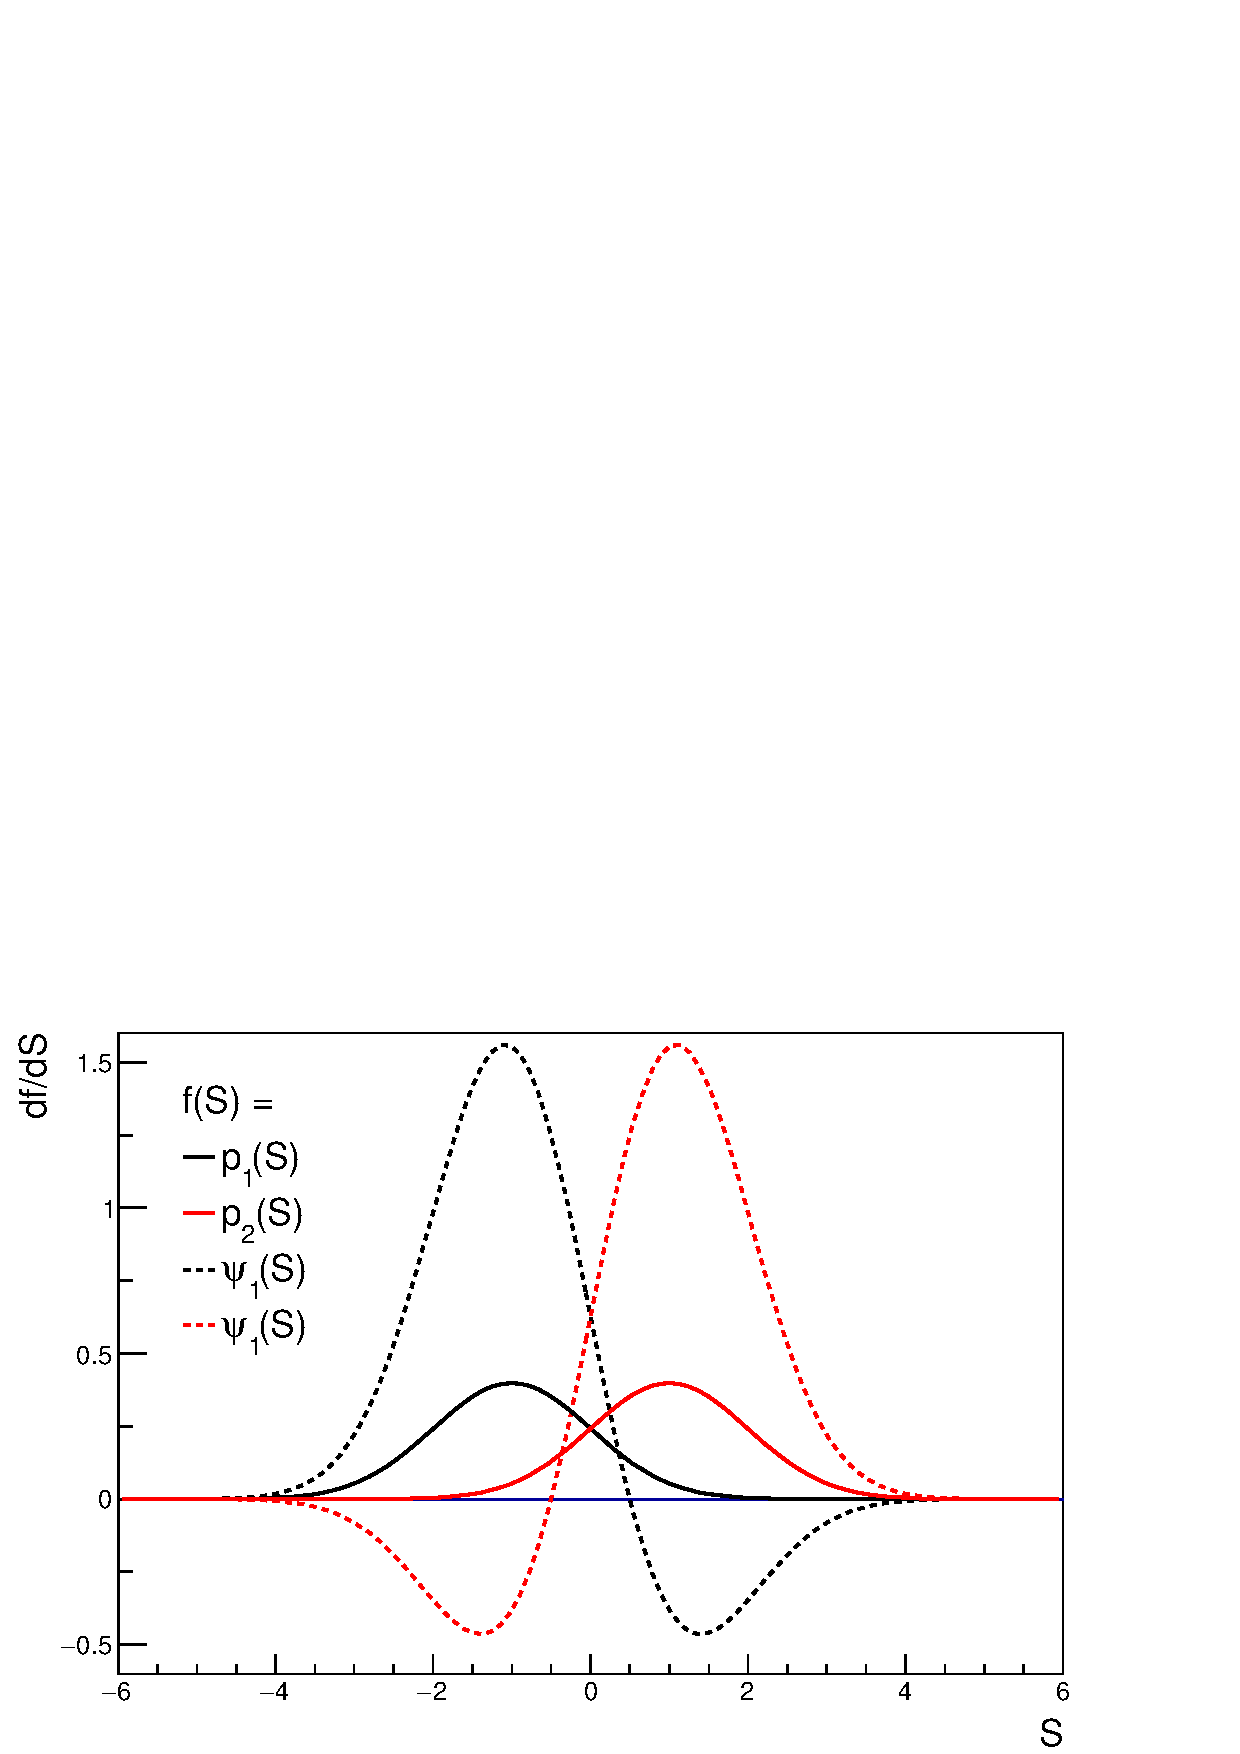
\includegraphics[width=0.7\textwidth]{../png/figGaus2.png}
\caption{Two Gaussian detector responses ($\Delta_{12} = 2$) and relative
  $\psi(S)$ amplitudes.}
\label{fig:Gaus2}
\end{figure}

\begin{figure}[!htb]
\centering
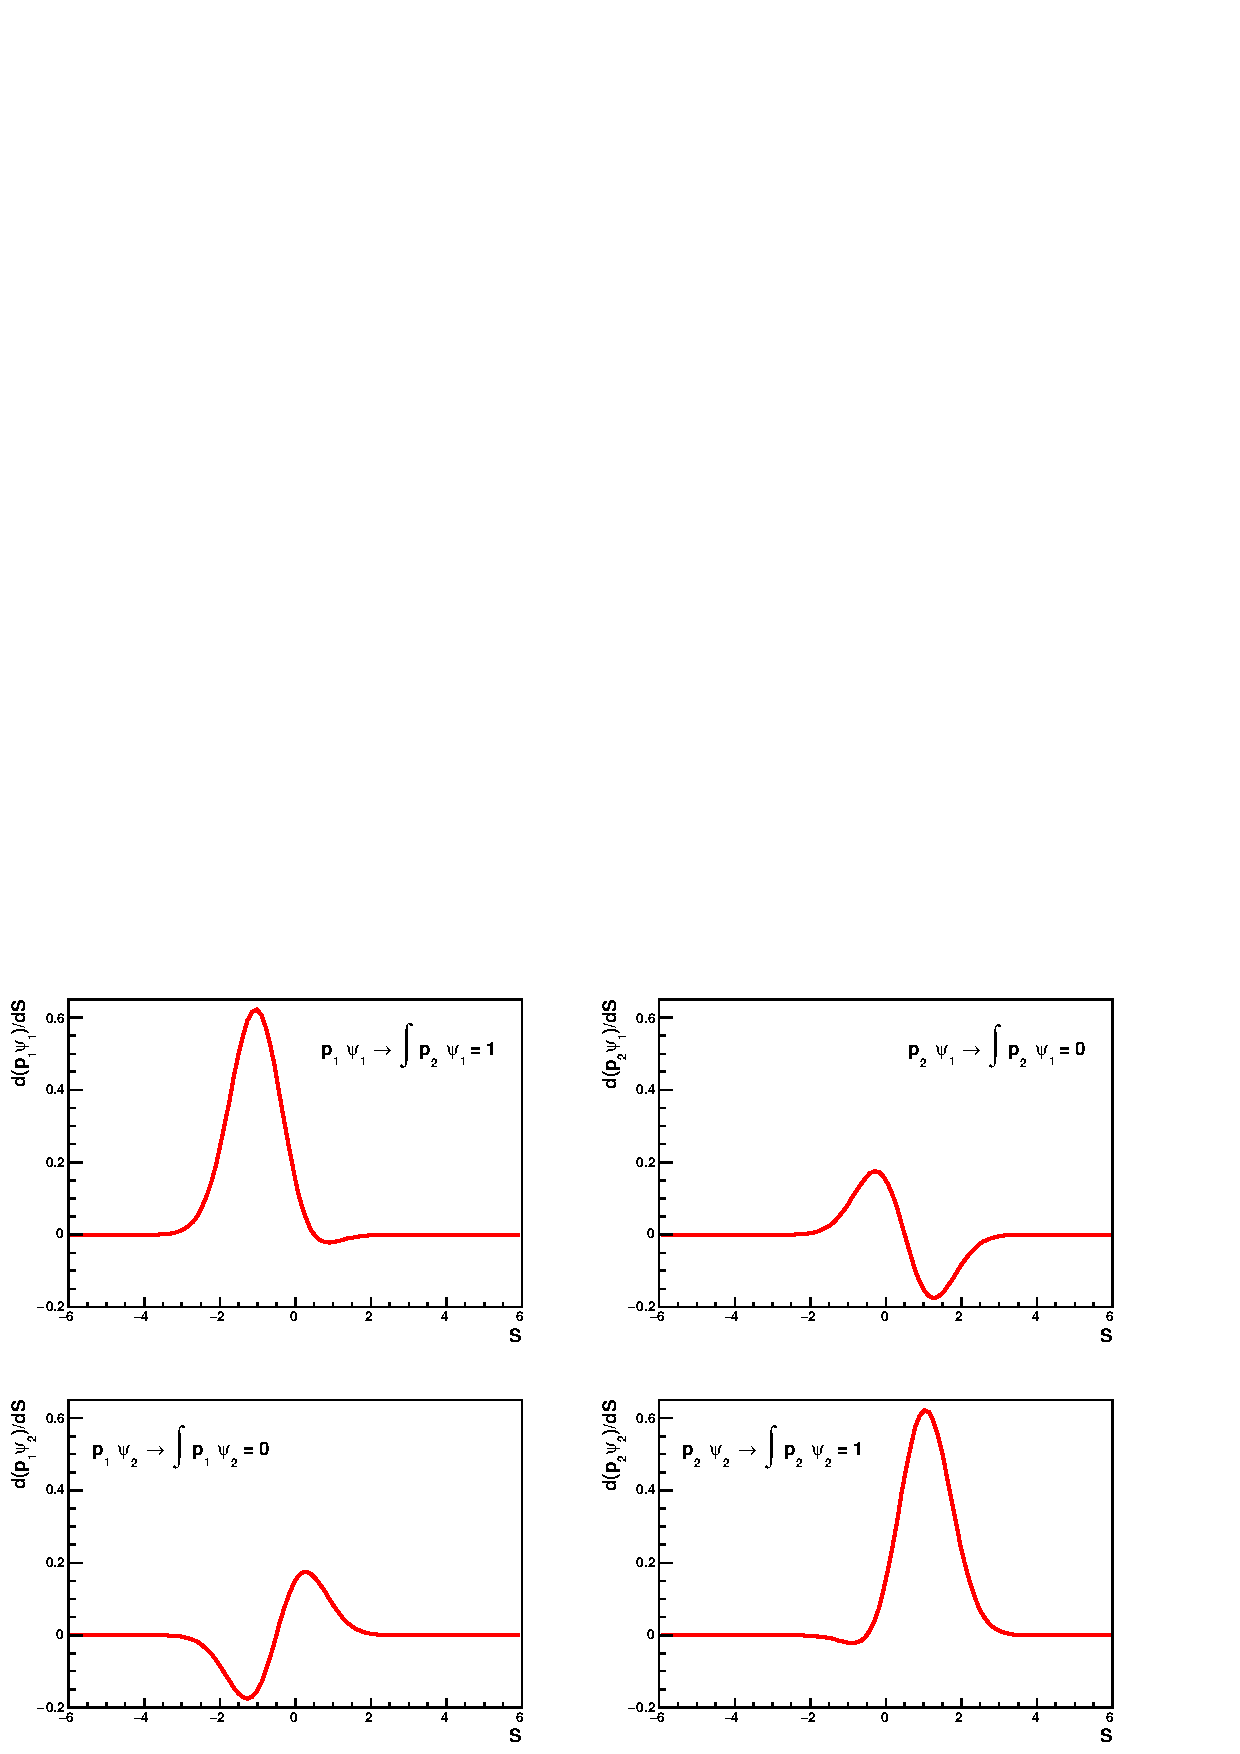
\includegraphics[width=0.7\textwidth]{../png/figSPgaus.png}
\caption{Scalar product functions for the two Gaussian responses case ($\Delta_{12} = 2$).}
\label{fig:Gaus2}
\end{figure}

\subsection{Combining both approaches}

\subsection{Multi-variables case}

\subsection{Correlations of event pair}



\section{Discussion}
\subsection{The effect of priors}

\subsection{Iterative vs analytical solutions}

\subsection{Advantages of the Bayesian approach}

\subsection{Advantages of the Quantum Mechanics formalism}



\input{conclusions}

%%%%%%%%%%%%%%%%%%%%%%%%%%%%     figure 5c  %%%%%%%%%%%%%%%%%%%%%%%%%
%\begin{figure}[!h]
%\begin{center}
%    \includegraphics[width=0.9\linewidth]{eps/plot_5.0_5.5.eps}
%\end{center}
%    \caption{$(N\sigma_{TPC},N\sigma_{TOF})$  distribution for all the species in 0-5\% PbPb collisions for $5.0 < p_{T} < 5.5~\rm{ GeV/}c$. The distributions were fitted assuming a Gaussian distribution plus exponential tail.}
%    \label{Fig:Nsigma2D3}
%\end{figure}
%%%%%%%%%%%%%%%%%%%%%%%%%%%%%%%%%%%%%%%%%%%%%%%%%%%%%%%%%%%%%%%%%%%%

\begin{thebibliography}{0}
%\bibitem{Adam:2015yta}  \BY{ALICE Collaboration (Adam, J. \etal)} \IN{Phys. Lett.}{B754}{2016}{360};

%\bibitem{} \BY{} \IN{}{}{}{};
%\bibitem{} \BY{} \IN{}{}{}{};
%\bibitem{} \BY{} \IN{}{}{}{};
%\bibitem{} \BY{} \IN{}{}{}{};
%\bibitem{} \BY{} \IN{}{}{}{};


%\bibitem{ref:apo} \BY{Einstein A. \atque Fermi E.}
%  \IN{Phys. Rev. A}{13}{1999}{12};
%  \SAME{69}{999}{1666}.
%\bibitem{ref:pul} \BY{Newton I.}
%  preprint INFN 8181.
%\bibitem{ref:bra} \BY{Bragg~B.}
%  \TITLE{Complete Works}, in \TITLE{Workers Playtime}, edited by \NAME{Tizio A. \atque Caio B.} (Unexeditor, Bologna) 1997, pp.~1-10.
\end{thebibliography}
\end{document}
